\section{}
National Institute of Nanotechnology (NINT) is a first generation Nano-research facility and the first of its kind in Canada. The facility is a six-storey building located on the University of Alberta Campus. Along with research offices, wet laboratories and clean nano-fab space, the facility features several ultra sensitive electron microscopes. In order for these microscopes to operate in the nanoscale, they must be provided with an extremely stable environment that is free from movement and vibration. One model of isolation setup for the electron microscopes is shown as (1) where an excitation displacement is applied to the base in response of floor vibration. The floor vibration is assumed to have a frequency of 50 Hz. The natural frequency of these whole setup is measured as 10 Hz.

\begin{figure}[h]
    \centering
    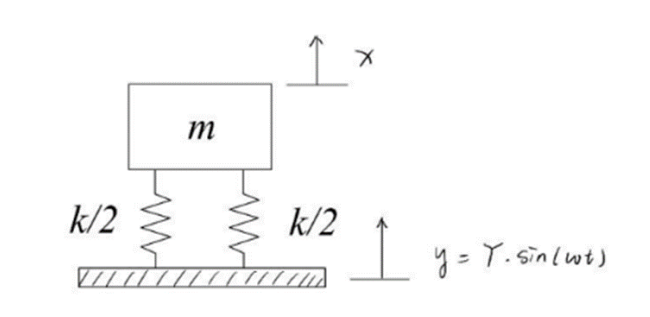
\includegraphics[width=0.5\textwidth]{Questions/Figures/q3 problem diagram.png}
\end{figure}

\begin{enumerate}[label=(\alph*)]
    \item (4 pts) Estimate the amplitude of vibration of electron microscope by comparing it to the amplitude of the floor for the setup as (1).
    \item (5 pts) The quality of the image from electron microscope is not satisfying since the amplitude is still too large. A dampler was added between the electron microscope and floor. What damping ratio should be chosen to make the amplitude of the vibration of electron microscope two times the amplitude in part a)?
    \item (1 pts) If the damping ratio of the damper needs to be adjusted to increase the amplitude of vibration of electron microscope, should the laboratory staff adjust the damping factor up or down?
\end{enumerate}

\subsection*{Solution}
\subsection{}
First, we decide the proper model for the problem. An appropriate model is an undamped SDOF system with base excitation. Since the springs are in parallel, the stiffness is $k_{\text{eff}} = k$. The DMF for this system is 
\begin{align*}
    \text{DMF} &= \frac{1}{1 - \left(\frac{\omega}{p}\right)^2}
\end{align*}
substituting,
\begin{align*}
    \text{DMF} &= \frac{1}{1 - \left(\frac{50}{10}\right)^2} \\
    &= \frac{1}{1 - 25} \\
    &= -0.04167
\end{align*}
This means that the amplitude of the electron microscope is $\boxed{4.167\%}$ of the amplitude of the floor. The negative sign indicated that the response of the electron microscope is 180 degrees out of phase with the floor.

\subsection{}
For a damped SDOF system with base excitation, the DMF is
\begin{align*}
    \text{DMF} &= \frac{\sqrt{1+\left(2\zeta\frac{\omega}{p}\right)^{2}}}{\sqrt{\left[1-\left(\frac{\omega}{p}\right)^{2}\right]^{2}+\left[2\zeta\frac{\omega}{p}\right]^{2}}}
\end{align*}
The DMF in a) was $1/24$, therefore we want the DMF to be $1/12$. 
\begin{align*}
    \frac{1}{12} &= \frac{\sqrt{1+\left(2\zeta\frac{50}{10}\right)^{2}}}{\sqrt{\left[1-\left(\frac{50}{10}\right)^{2}\right]^{2}+\left[2\zeta\frac{50}{10}\right]^{2}}} 
\end{align*}
Solving for $\zeta$,
\begin{verbatim}
syms zeta
eqn = 1/12 == sqrt(1+(2*zeta*5)^2)/sqrt((1-(5)^2)^2+(2*zeta*5)^2);
zeta = solve(eqn, zeta);
zeta = double(zeta)

>> zeta =
        -0.1738
         0.1738
\end{verbatim}
Therefore, the damping ratio should be $\boxed{0.1738}$.

\subsection{}
\begin{figure}[h]
    \centering
    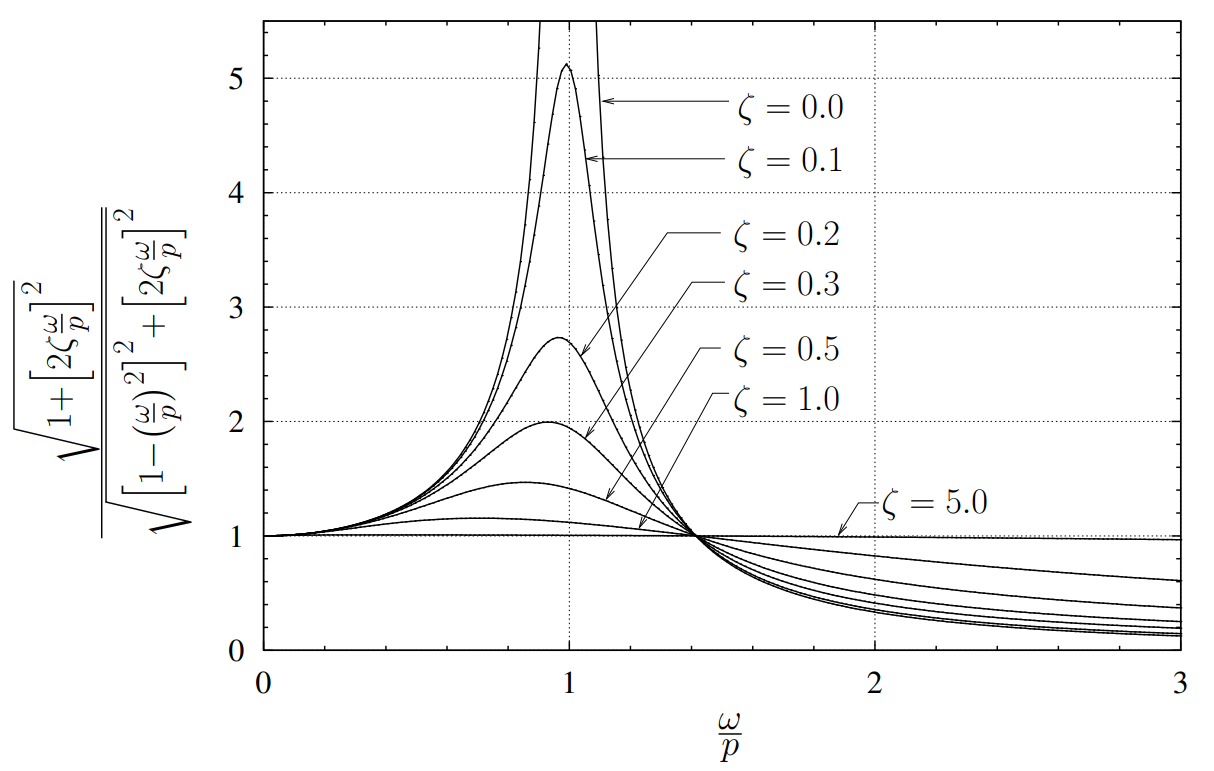
\includegraphics[width=0.5\textwidth]{Questions/Figures/q3 dmf diagram.png}
    \caption{Response amplitude of damped spring–mass system subjected to harmonic base
    excitation}
\end{figure}
Since we are operating on the RHS of the resonance peak, we should adjust the damping factor \textbf{up} to increase the amplitude of vibration of the electron microscope.